% vim: spell spelllang=en_us
\documentclass[conference,11pt]{IEEEtran}
\usepackage[T1]{fontenc}
\usepackage[utf8]{inputenc}
\usepackage[english]{babel}
\usepackage{csquotes}
\usepackage{biblatex}
\usepackage{amsmath}
\usepackage{amsthm}
\usepackage{amssymb}
\usepackage{listings}
\usepackage{minted}
\usepackage{tipa}
\usepackage{mdframed}
\usepackage[inline]{enumitem}
\usepackage{environ}
\usepackage{varioref}

\addbibresource{../references.bib}

\MakeOuterQuote{"}
\setminted{autogobble,python3,mathescape,frame=lines,framesep=2mm,fontsize=\footnotesize,escapeinside=||}
\renewcommand\listingscaption{Query Set}

\NewEnviron{equations}{%
\begin{equation}\begin{split}
    \BODY
\end{split}\end{equation}
}

\usepackage{pgfplots}
\pgfplotsset{compat=newest}

\newtheorem{definition}{Definition}

\title{%
    Applications and Implementation of Differential Privacy on Statistical
    Databases
}
\author{%
    \IEEEauthorblockN{%
        Jonathan Sumner Evans\IEEEauthorrefmark{1},
        Victoria Girkins\IEEEauthorrefmark{2}, and
        Sam Sartor\IEEEauthorrefmark{3}
    }
    \IEEEauthorblockA{%
        Department of Computer Science,
        Colorado School of Mines\\
        Golden, Colorado\\
        Email:
            \IEEEauthorrefmark{1}jonathanevans@mines.edu,
            \IEEEauthorrefmark{2}vgirkins@mines.edu,
            \IEEEauthorrefmark{3}ssartor@mines.edu,
    }
}

\begin{document}
\maketitle
\thispagestyle{plain}
\pagestyle{plain}

% (1) an abstract
\begin{abstract}
    Statistical databases have long been known to be vulnerable to inference
    attacks.  We describe the nature of inference attacks and analyze one
    method, called Differential Privacy, of mitigating these attacks. We discuss
    two mechanisms for Differential Privacy. We then explain our implementation
    of a simple Differential Privacy statistical database and the experiments we
    performed on the database. Then, we analyze how well our implementation
    achieves the objectives of Differential Privacy databases. We conclude by
    calling on industry to create differential privacy implementations that can
    be used in general applications.
\end{abstract}

% (2) introduction (including the background, motivation, and goal)
\section{Introduction}
Statistical databases are designed for statistical analysis of the datasets
contained within the database. One of the desired properties of statistical
databases is that nothing about an individual should be learnable from the
database that cannot be learned without access to the
database~\cite{Dwork:2006:DP}. In other words, gathering information about the
individual records using allowed queries on the database should be impossible.

Without any protections, well-crafted queries to a statistical database can
implicitly reveal private information.  Such an attack is know as an
\textit{inference attack}.  To understand these attacks, one must consider the
case of two databases which differ by only a single row.  Consider, for example,
a database which associates people with their incomes.  The query

\begin{minted}{sql}
    SELECT SUM(income) FROM table
\end{minted}
seems harmless at first. But if a new record were added and we ran the query
again, the difference between the two results would represent the exact income
of the new entry. If the attacker knows the identity of the person who was
added, the privacy leak becomes even more severe.

Of course, an attacker may not have the luxury of always knowing when a new
record will be added to the database, and of timing his queries accordingly. He
may, however, achieve the same results by narrowing down his query with
conditionals.

The query
\begin{minted}{sql}
    SELECT SUM(income)
      FROM table
     WHERE zip != 80127
\end{minted}
may be sufficient in a small-enough database; in a larger database, an attacker
may need to add more conditionals to ensure the queries jointly isolate a single
row.  However, since the danger occurs when information about a single entry is
returned, regardless of how the attacker managed it, we will assume for
simplicity's sake that the database is queried before and after the addition of
a single row.

\subsection{Previous Attempts at Anonymizing Statistical Data}
Attempts have been made to privatize data in the past and many are still in use
today. However, everything from simply removing columns containing sensitive
information to advanced techniques such as as k-anonymity and l-diversity have
been shown to be vulnerable to attack~\cite{Atockar:2014}.  K-anonymity, for
example, does not include any randomization and thus attackers can still make
inferences about data sets~\cite{Aggarwal:2005}.

\subsection{Differential Privacy}
In 2006, Cynthia Dwork, a researcher at Microsoft, proposed a new technique to
reduce the risk of a successful inference attack called \textit{Differential
Privacy}~\cite{Hilton:DP:history}. The goal of Differential Privacy is to
maximize the statistical accuracy of queries on a statistical database while
also maximizing the privacy of the individual records. It does this by
introducing noise into the dataset. This randomness reduces the likelihood of
obtaining meaningful information about the individual records in the database.

The real power of Differential Privacy is achieved when it is used in
conjunction with a privacy bound, $\varepsilon$, as described in
Section~\ref{sec:epsilon-dp}. We discuss the methods for generating random noise
in Section~\ref{sec:dp-mech}. In Section~\ref{sec:using-laplace-dp}, we explain
details about how the one of the mechanisms is used to ensure differential
privacy.

\subsubsection{Epsilon-Differentially Private}\label{sec:epsilon-dp}
One useful way of discussing Differential Privacy is to talk about what it means
for a database to be \textit{epsilon-differentially private}. A database falls
under this category if it is private as bounded by a chosen value epsilon. As
opposed to the mathematical definition, here we give a more intuitive definition
as stated by Atockar~\cite{Atockar:2014}:

\blockquote{%
    This [epsilon-differentially private] can be translated as meaning that the
    risk to one's privacy should not substantially (as bounded by epsilon)
    increase as a result of participating in a statistical database.
}

For the sake of rigorousness, the formal mathematical definition of
epsilon-differential privacy described by Dwork~\cite{Dwork:2006:DP} follows.

\begin{mdframed}
    \begin{definition}
        A randomized function $\mathcal{K}$ gives
        \textbf{\textepsilon-differential privacy} if for all data sets $D$ and
        $D'$ differing on at most one row, and all $S \subseteq
        Range(\mathcal{K})$,
        \begin{equation}
            \Pr[\mathcal{K}(D) \in S] \leq \exp(\varepsilon) \times
            \Pr[\mathcal{K}(D') \in S]
        \end{equation}
    \end{definition}
\end{mdframed}

For now, all that concerns us about this equation is that $D$ and $D'$ are the
earlier-mentioned databases differing by a single row, and $\mathcal{K}$ is our
mechanism for adding noise drawn from our distribution as described in
Section~\ref{sec:dp-mech}.

\subsubsection{Differential Privacy Mechanisms}\label{sec:dp-mech}
There are two primary Differential Privacy Mechanisms: the Exponential Mechanism
and the Laplace Mechanism. The Exponential Mechanism should be used on
categorical, non-numeric data. For example, queries of the form ``What is the
most common eye color in this room?'' should be protected using the Exponential
Mechanism~\cites{Atockar:2014}[8]{Roth:2011:DP-exp}. The Laplace Mechanism
should be used with non-categorical, real-value data~\cite{Geng:2014}. Because
of the nature of our data, our primary focus for this project is the Laplace
Mechanism.

Before we rigorously examine the mathematics, let us review our inputs and our
goals:

\begin{itemize}[leftmargin=4em]
    \item [\textbf{Inputs}] A statistical database with sensitive information,
        an attacker poised with a malicious query, and a desired epsilon, or
        privacy parameter.

    \item [\textbf{Goals}] To add enough Laplace-distributed noise to the
        results of database queries that our database is mathematically
        considered differentially private.
\end{itemize}

Mathematically, the Laplace Distribution is defined as follows:
\begin{mdframed}
    \begin{definition}\label{def:laplace}
        The \textbf{Laplace Distribution}, $\text{Lap}(\mu, b)$, also known as a
        symmetric exponential distribution, is the probability distribution with
        p.d.f.:
        \begin{equation}
            P(x|\mu, b) = \frac{1}{2b}\exp\left(-\frac{|x - \mu|}{b}\right)
        \end{equation}
        where $\mu$ is the location of the center of the distribution and $b$ is
        the scale parameter.

        Figure~\ref{fig:laplace-pdf} is a visualization of the p.d.f.\ for a few
        values of $\mu$ and $b$.\\

        \begin{figure}[H]
            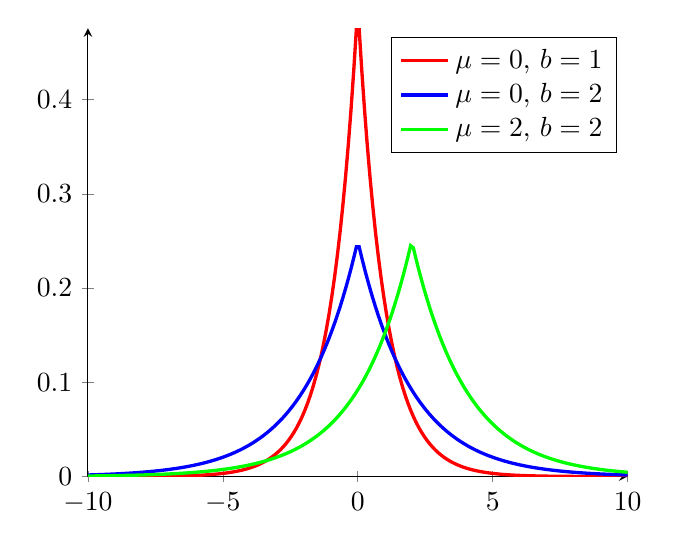
\begin{tikzpicture}
                \begin{axis}[axis lines = left]
                    \addplot [domain=-10:10, samples=200, color=red, very thick]
                    {(1 / 2) * exp(-abs(x))};
                    \addlegendentry{$\mu=0$, $b=1$}
                    \addplot [domain=-10:10, samples=200, color=blue, very thick]
                    {(1 / (2 * 2)) * exp(-abs(x) / 2)};
                    \addlegendentry{$\mu=0$, $b=2$}
                    \addplot [domain=-10:10, samples=200, color=green, very thick]
                    {(1 / (2 * 2)) * exp(-abs(x - 2) / 2)};
                    \addlegendentry{$\mu=2$, $b=2$}
                \end{axis}
            \end{tikzpicture}
            \caption{Probability Density Function for the Laplace Distribution}
            \label{fig:laplace-pdf}
        \end{figure}
    \end{definition}
\end{mdframed}

For us, $\mu$ is 0; we can use the Zero-Centered Laplace Distribution, which has
only one parameter, $b$, the scale.

To draw a value from the Zero-Centered Laplace Distribution efficiently, we use
the random variate for the Laplace Distribution which is defined as follows:
\begin{mdframed}
    \begin{definition}\label{def:laplace-variate}
        The \textbf{Laplace Random Variate} is
        \begin{equation}
            X(u) =
                \begin{cases}
                    -b \log|u| & \text{if }u > 0\\
                    b \log|u| & \text{if }u \leq 0
                \end{cases}
        \end{equation}
        where $u$ is uniformly distributed in the range $(-1, 1)$.
    \end{definition}
\end{mdframed}

\subsubsection{Using the Laplace Differential Privacy Mechanism}\label{sec:using-laplace-dp}
In choosing the value for $b$, it makes sense that we should consider
\textepsilon, which quantifies the level of privacy we desire. Another factor
comes into play, however: the "sensitivity" of the database. This is defined as
the maximum difference between the results of any query run on two databases
which differ by only one row, as described above~\cite{Atockar:2014}. We shall
assume
\begin{minted}{sql}
    SELECT SUM(income) FROM table
\end{minted}
is the only query that this database will accept, so the "sensitivity" of our
database is clearly the highest income in the table, since this value will be
the difference between two queries run on the database before and after the
record associated with this income is added.

So, we must add noise while considering both {\textepsilon} and the database's
above-defined sensitivity. In fact, in a paper by
Dwork~\cite{Dwork:2011:private-data-analysis}, it was proven that choosing the
"scale" parameter ($b$) of our Laplace distribution according to the equation
\begin{equation}
    b = {\Delta}f/\varepsilon
\end{equation}
where ${\Delta}f$ is sensitivity, our database will mathematically satisfy
epsilon-differential privacy. That is, we should add noise to the data drawn
from a 0-centered Laplace distribution with scale parameter
${\Delta}f/\varepsilon$.

A further consideration we must make is the possibility of multiple queries to
the database. The Laplace distribution is symmetrical, so if unlimited queries
were allowed, the attacker could simply run his query many times and take the
average to extract sensitive data. So we must limit the number of queries
allowed; fortunately, the calculation is linear. Assume we draw all noise from
the same distribution (it would be possible to vary it but this unnecessarily
complicates things), and that this distribution is Laplace, 0-centered, with a
privacy parameter $\varepsilon_i$ (that is, with scale parameter
${\Delta}f/\varepsilon_i$). If we limit learners to $k$ queries, our overall
privacy budget is $k\varepsilon_i$. This privacy budget is our actual epsilon;
as stated by Atockar, "it reflects the maximum privacy release allowable for the
total query session"~\cite{Atockar:2014}.

So to sum it up practically: if we wish to make our database
epsilon-differentially private as bounded by some value epsilon; our database
has sensitivity ${\Delta}f$; and we wish for learners to be allowed $k$ queries
before being locked out; we should add a random variable to each query, drawn
from the 0-centered Laplace distribution with scale parameter $k \times
{\Delta}f/\varepsilon$.

Of course, the lower of a privacy budget we allow, the noisier the data returned
by the queries will become~\cite{Atockar:2014}. If our queries become useless
due to the noise in the data, we may choose to raise the privacy budget (that
is, to increase the value of epsilon) or to further limit the number of queries
each user is allowed (that is, to lower the value of $k$). As with many issues
in information security, this is a balancing act between security and usability;
we should consider the nature of the database, its contents, and its purpose
when choosing where to draw this line.

\begin{center}***\end{center}

For our final project, we implemented and analyzed a Differential Privacy
database which can perform a limited set of aggregate functions on a dataset.
We describe our database implementation in Section~\ref{sec:db-impl}. Our
experiment is explained in Section~\ref{sec:experiment}. The results of our
experiment are summarized in Section~\ref{sec:results} and we discuss some of
the limitations of our implementation in Section~\ref{sec:limitations}. In
Section~\ref{sec:future-work} we describe some of the potential future work in
the field of Differential Privacy. We conclude in Section~\ref{sec:conclusion}
and call on industry to create effective, easy-to-use Differential Privacy
implementations for inclusion in general industry applications.

% (3) key idea and approach (e.g., survey, testbed, system
% design/implementation, experiments, etc.)
\section{Database Implementation}\label{sec:db-impl}
% reads CSV
Our actual database implementation was written in Python to speed up development
time. If we were implementing this in an application that needed high
performance, we would use a compiled language such as C or Rust.  To help us
test our implementation, we designed our database to allow the user to enable
and disable Differential Privacy. When Differential Privacy is enabled, the user
is also able to configure {\textepsilon} and the query limit.

The database reads the data from a CSV file which is specified by the user and
then allows the following aggregate, or summary, functions on the data:
\begin{itemize}
    \item \textbf{\texttt{SUM}}: the numerical sum of the values in a column
    \item \textbf{\texttt{COUNT}}: the number of rows
    \item \textbf{\texttt{MIN}}: the minimum numerical value in the column
    \item \textbf{\texttt{MAX}}: the maximum numerical value in the column
    \item \textbf{\texttt{MEAN}}: the average value in the column
    \item \textbf{\texttt{VARIANCE}}: the statistical variance of the column
    \item \textbf{\texttt{SD}}: the standard deviation of the column
\end{itemize}

% How to compute statistic (e.g. mean = total / count)
We describe how we calculate these statistics and how we find $\Delta f$ for
each of these functions in Section~\ref{sec:summary-functions}.

% Where clause
Our database implementation allows the user to specify a \texttt{WHERE} clause.
Currently, we implement this as a directly evaluated Python expression which is
executed via the \texttt{eval} function in Python. This is a code injection
vulnerability, but our goal is to study Differential Privacy, not code injection
prevention. Future iterations of our project could wrap this functionality and
prevent code injection attacks.

Our implementation also handles edge cases where zero or one row is returned to
avoid divide-by-zero errors.  For most statistics, in the case when one row is
returned, we merely use the value of that row as the sensitivity of the query.
For the case when zero rows are returned, we add a fake entry whose value is the
mean of the column and then handle it like the one row case. Future iterations
of our project could improve the robustness of our edge case handling.

The statistic and $\Delta f$ are calculated using the functions described in
Section~\ref{sec:summary-functions}. Noise is added according to the Laplace
Distribution as described in Section~\ref{sec:using-laplace-dp}. This privatized
result is then displayed. For testing purposes, we also output the actual
statistic, but this can easily be removed in future implementations.

\subsection{Summary Functions}\label{sec:summary-functions}
In this section, we define each of the summary functions $f$ over the set of
values $D$. We also define the sensitivity $\Delta f$ for each summary function.
\begin{mdframed}
    \begin{definition}
        For any statistic $f(D)$, the \textbf{sensitivity of a query}, $\Delta
        f(D)$, is defined as follows:
        \begin{equation}
            \Delta f(D) = \left|f(D) - f(D')\right|
        \end{equation}
        where $D' \subset D$, $|D'| = |D| - 1$, and $D'$ maximizes $\Delta
        f(D)$.
    \end{definition}
\end{mdframed}

Generally, $\Delta f(D)$ can be found by iterating over all possible $D'$ and
finding the maximum $|f(D) - f(D')|$. This brute force algorithm often has
$\mathcal{O}(n^2)$ complexity and is very slow on large datasets. To allow for
more performant queries, our implementation individually defines $f$ and $\Delta
f$ for each of the following summary functions.

\subsubsection{Count}
Removing any one row from the dataset decreases the row count by one. Thus,
sensitivity of count is always 1.
\begin{equations}
    \text{count}(D) &= |D| \\
    \Delta\text{count}(D) &= 1
\end{equations}

\subsubsection{Sum}
The largest element in a set has the most influence on the set's sum. Thus the
sensitivity of the statistic is always the maximum $d \in D$.
\begin{equations}
    \text{sum}(D) &= \sum{D} \\
    \Delta\text{sum}(D) &= \max(D)
\end{equations}

\subsubsection{Mean}
Mean is most changed by the addition or removal of elements with a high variance
from the mean. Let $d$ be some $d \in D$ where $|d - \text{mean}(D)|$ is
maximal. Then
\begin{equations}
    \text{mean}(D) &= \frac{\sum D}{|D|} \\
    \Delta\text{mean}(D) &= \left| \frac{\sum D}{|D|} - \frac{\sum (D) - d}{|D| - 1} \right|
\end{equations}

\subsubsection{Maximum}
Let $l_n$ be the $n^\text{th}$ largest element in $D$. Since $\max(D)$ is
dependent only on $l_0$, $D'$ must not contain $l_0$.
\begin{equations}
    \max(D) &= l_0 \\
    \Delta\max(D) &= l_0 - l_1
\end{equations}

\subsubsection{Minimum}
Let $s_n$ be the $n^\text{th}$ smallest element in $D$. Since $\min(D)$ is
dependent only on $s_0$, $D'$ must not contain $s_0$.
\begin{equations}
    \min(D) &= s_0 \\
    \Delta\min(D) &= s_1 - s_0
\end{equations}

\subsubsection{Variance \& Standard Deviation}
We use the brute force method for these functions. A more efficient method
certainly exists, but we have not yet implemented it.

% Have to include this table here so it shows up on the next page
\begin{table*}[h]
    \caption{Columns in Our Sample Dataset}\label{tab:cols}
    \centering
    \begin{tabular}{l | l | l}
        \textbf{Field} & \textbf{Column Name} & \textbf{Generation Method} \\
        \hline
        Name & \texttt{name} & the \texttt{names} Python library \\
        Age & \texttt{age} & uniformly distributed between 18 and 65 \\
        Income & \texttt{income} & distributed log-normal \\
        Zip Code & \texttt{zip} & from a random set of \textasciitilde40
            five-digit numbers \\
        Net-worth & \texttt{net\_worth} & from age, income, and a random offset
    \end{tabular}
\end{table*}

% (4) activities (such as literature study and experiments) that you performed
\section{Experiment}\label{sec:experiment}
To perform our experiment, we generated a large sample dataset suitable for
statistical queries (Section~\ref{sec:dataset}). We used the database that we
implemented in Section~\ref{sec:db-impl} and crafted a set of queries with which
to attack our database (Section~\ref{sec:crafted-queries}).

\subsection{Dataset}\label{sec:dataset}
To test our database, we created a dataset with 10,000 data points (rows). The
columns for each row are listed in Table~\vref{tab:cols}.  The dataset was
generated using a Python program and is output to a comma separated value (CSV)
file. We chose to use a CSV file for simplicity; however, future iterations of
our project could use a more sophisticated data store.

We chose the generation methods to roughly model the distributions of names,
age, income, zip code, and net worth of the US population. For example, the
income is distributed log-normal which approximates the distribution of incomes
in the United States.

\subsection{Crafted Queries}\label{sec:crafted-queries}
After generating our dataset, we crafted a set of queries that would to test the
effectiveness of our Differential Privacy database implementation. We provide a
small sample of queries here to demonstrate the properties of our Differential
Privacy database. Because we have access to the underlying data, we were able to
craft these queries with inside knowledge. Although our database does not parse
SQL queries, we will use SQL here for clarity. Each set of queries targets an
individual's sensitive information. The sets of queries we created were as
follows. (Note, \texttt{table} is the single table that we created in
Section~\ref{sec:dataset}.)

\begin{listing}[H]
    \begin{minted}{sql}
        SELECT SUM(age)     SELECT SUM(age)
          FROM table          FROM table
         WHERE zip = 31643   WHERE zip = 31643
                               AND name != "Abel Woods"
    \end{minted}
    \caption{Identifying Abel Woods' Age}
    \label{qs:abel}
\end{listing}

\begin{listing}[H]
    \begin{minted}{sql}
        SELECT MEAN(age)
          FROM table
          WHERE net_worth + 1 >
            (SELECT MAX(net_worth) FROM table)

        SELECT MEAN(income)
          FROM table
          WHERE net_worth + 1 >
            (SELECT MAX(net_worth) FROM table)
    \end{minted}
    \caption{Identifying the age and income of the richest person}
    \label{qs:richest-person}
\end{listing}

\begin{listing}[H]
    \begin{minted}{sql}
        SELECT COUNT(name)
            FROM table
            WHERE name == "Peter Gist"
    \end{minted}
    \caption{Discovering if Peter Gist is in the database}
    \label{qs:peter}
\end{listing}

% (5) description and analysis of the key results and observations
\section{Results}\label{sec:results}
After creating a dataset, implementing a database, and choosing a set of queries
with which to test the database, we performed our experiment. We ran each of the
queries on the dataset with Differential Privacy disabled, and then with
Differential Privacy enabled, and compared the results.

\subsection{Query Set~\ref{qs:abel}}

With Differential Privacy disabled, our database implementation output for the
first query set is as follows.
\begin{minted}{html}
    use dp (y/n): |$\text{\textbf{\texttt{n}}}$|
    database csv: bigdata.csv
    =================
    summarize field: age
    summary function: sum
    where: zip == 31643
    |$\text{\textbf{\texttt{10412}}}$|
    =================
    summarize field: age
    summary function: sum
    where: zip == 31643 and name != "Abel Woods"
    |$\text{\textbf{\texttt{10379}}}$|
\end{minted}
From this set of  queries, we can determine that the total age of the people in
ZIP code 31643 is 10412; this is not a privacy violation. However, we can also
infer that Abel Woods is $10412 - 10379 = 33$ years old. This is a violation of
privacy.

With Differential Privacy enabled, the output is as follows.
\begin{minted}{html}
    use dp (y/n): |$\text{\textbf{\texttt{y}}}$|
    epsilon: 5
    query limit: 2
    database csv: bigdata.csv
    =================
    summarize field: age
    summary function: sum
    where: zip == 31643
    |$\text{\textbf{\texttt{10409}}}$|
    =================
    summarize field: age
    summary function: sum
    where: zip == 31643 and name != "Abel Woods"
    |$\text{\textbf{\texttt{10435}}}$|
\end{minted}
From this set of queries, we determine that the total age of the people in ZIP
code 31643 is 10409, a 0.2\% error. If we attempt to use these queries to find
the age of Abel Woods we will get $10409 - 10445 = 49$, a 48\% error. We can see
that with Differential Privacy enabled, Abel Woods' privacy is protected, but
summary queries on the database still return useful information.

\subsection{Query Set~\ref{qs:richest-person}}
With Differential Privacy disabled, our database implementation output for the
first query set is as follows.
\begin{minted}{html}
    use dp (y/n): |$\text{\textbf{\texttt{n}}}$|
    database csv: bigdata.csv
    =================
    summarize field: net_worth
    summary function: max
    where: True
    |$\text{\textbf{\texttt{5246937}}}$|
    =================
    summarize field: income
    summary function: mean
    where: net_worth > 5246936
    |$\text{\textbf{\texttt{304322}}}$|
    =================
    summarize field: age
    summary function: mean
    where: net_worth > 5246936
    |$\text{\textbf{\texttt{65}}}$|
\end{minted}
From these queries, we can determine that the richest person in the database has
a net worth of \$5,246,937. Using this person's net worth, we can filter our
queries to only this person and can then determine the income (\$304,233) and
age of this person (65). This is the true age and income of the richest person
and thus is an obvious breach of privacy.

With Differential Privacy enabled, the output is as follows.
\begin{minted}{html}
    use dp (y/n): |$\text{\textbf{\texttt{y}}}$|
    epsilon: 3
    query limit: 3
    database csv: bigdata.csv
    =================
    summarize field: net_worth
    summary function: max
    where: True
    # stat=5246937 b=1332431
    |$\text{\textbf{\texttt{3900194}}}$|
    =================
    summarize field: income
    summary function: mean
    where: net_worth > 3900194
    # stat=275988 b=28335
    |$\text{\textbf{\texttt{240135}}}$|
    =================
    summarize field: age
    summary function: mean
    where: net_worth > 3900194
    # stat=63 b=2
    |$\text{\textbf{\texttt{62}}}$|
\end{minted}
Here, the maximum net worth is protected. There is a massive discrepancy between
the returned maximum net worth and the actual max net worth. This is because
maximums are very sensitive; they reflect only the most extreme data points. As
a result, a large amount of randomness must be added to protect them.  In this
instance, the $\Delta f$ value is over \$1.3 million resulting in a 25\% error.

Queries on income and age return fairly accurate results, but this is only due
to the fact that the lower net worth caused us to match two different
individuals, both of whom were wealthy and in their sixties. However, the
richest person's privacy is still safe.

\subsection{Query Set~\ref{qs:peter}}
With Differential Privacy disabled, our database implementation for the third
query set is as follows.
\begin{minted}{html}
    use dp (y/n): |$\text{\textbf{\texttt{n}}}$|
    database csv: bigdata.csv
    =================
    summarize field: name
    summary function: count
    where: name == "Peter Gist"
    |$\text{\textbf{\texttt{1}}}$|
    =================
    summarize field: name
    summary function: count
    where: name == "Foo Bar"
    |$\text{\textbf{\texttt{0}}}$|
\end{minted}
From these queries, we cannot determine whether Peter Gist or Foo Bar exist 
in the database.

With Differential Privacy Enabled, the output is as follows.
\begin{minted}{html}
    use dp (y/n): |$\text{\textbf{\texttt{y}}}$|
    epsilon: 4
    query limit: 4
    database csv: bigdata.csv
    =================
    summarize field: name
    summary function: count
    where: name == "Peter Gist"
    # stat=1 b=1
    |$\text{\textbf{\texttt{-3.10}}}$|
    =================
    summarize field: name
    summary function: count
    where: name == "Peter Gist"
    # stat=1 b=1
    |$\text{\textbf{\texttt{0.63}}}$|
    =================
    summarize field: name
    summary function: count
    where: name == "Foo Bar"
    # stat=0 b=1
    |$\text{\textbf{\texttt{-2.23}}}$|
    =================
    summarize field: name
    summary function: count
    where: name == "Foo Bar"
    # stat=0 b=1
    |$\text{\textbf{\texttt{1.15}}}$|
\end{minted}
From these queries, we can infer nothing about whether or not Peter Gist and
Foo Bar exist in the database.

% (6) discussion of the limitations and potential future work
\section{Limitations}\label{sec:limitations}
Our Differential Privacy implementation is limited. Some of the limitations
include:
\begin{itemize}
    \item Our implementation does not parse actual SQL queries. However, we
        have designed our program in a way that makes it easy to add a parsing
        engine on top of our program.
    \item Our implementation supports a very limited set of SQL operations. For
        example, it does not support \texttt{join} statements.  Future
        iterations of this project could implement more of the SQL standard.
    \item Our implementation can only process numerical data and is limited to
        the Laplace Mechanism. Adding alternative Differential Privacy
        mechanisms, such as the Exponential Mechanism, would greatly improve the
        practicality of our Differential Privacy implementation.
    \item Our implementation is not heavily optimized. Currently, some queries
        have $\mathcal{O}(n^2)$ algorithmic complexity. In further iterations of
        our implementation, we could improve the performance of our system by
        using caching methods and by optimizing our algorithms.
    \item Our code base is not particularly extensible. Future implementations
        could improve the software design to make it adhere to good software
        engineering principles.
    \item We did not do any research regarding the proper handling of these edge
        cases where one or zero rows match the query. Our implementation seems
        to protect the privacy of individuals in these cases as shown by Query
        Set~\ref{qs:peter}. However, we have no research to back up the validity
        of our approach, and thus there may be some vulnerabilities in our
        implementation.
\end{itemize}

Although our Differential Privacy implementation is not complete, our experiment
proved that it was extremely effective at protecting the privacy of the
individual records in the database.

\section{Future Work}\label{sec:future-work}
Differential Privacy is a relatively new method of protecting data in a
statistical database. As such, there are not many implementations of it outside
of academia and large companies like Microsoft and Apple. If differential
privacy were adopted by a larger percentage of the industry, more statistical
databases with sensitive information would be resistant to inference attacks.

Software engineers have a great opportunity to create implementations of
Differential Privacy suitable for use in general industry applications. Such an
implementation could be a library which other programmers could include in their
project using dependency managers such as \texttt{pip}, \texttt{npm}, or
\texttt{cargo}. The creation of these general-purpose libraries could help make
Differential Privacy more accessible and cost-effective for industry
professionals. This would help increase adoption of Differential Privacy, and
would result in an overall improvement of users' privacy in the industry.

% (7) conclusion
\section{Conclusion}\label{sec:conclusion}
Before starting on this project, our understanding of Differential Privacy was
very limited. We expected that we would need to parse each query and handle a
large number of cases to ensure the privacy of the data.  After significant
research, we found implementing of Differential Privacy would not require
significant query parsing or edge-case handling. We were surprised by the
mathematical rigor of Differential Privacy.

Even with our implementation of a simple Differential Privacy solution, we were
able to demonstrate its effectiveness at protecting users' privacy. Despite its
usefulness, Differential Privacy has not seen significant adoption in industry
outside of large companies. Thus, we take this opportunity to call on industry
to create Differential Privacy libraries that are suitable for use in general
industry applications. We believe that if such libraries are created, the
privacy of user data throughout the industry will be vastly increased.

% (8) references
{\printbibliography}

\end{document}
